\section{Atomes de Rydberg en interaction}
Dans cette thèse, nous allons nous intéresser aux interactions entre plusieurs atomes de Rydberg voisins, dans des niveaux identiques ou proches en énergie.
Le reste de ce chapitre est consacré au calcul de ces interactions et à leur application aux deux cas qui nous concernent : autour des niveaux 60S et 50C.

	\subsection{Deux atomes de Rydberg qui se parlent}
L'opérateur de moment dipolaire entre deux niveaux de Rydberg proches est grand, comme nous l'avons évoqué.
En cela, les atomes de Rydberg sont de très bonnes antennes pour le rayonnement électromagnétique lorsque celui-ci est résonant avec les fréquences de transition entre niveaux proches.
Cette caractéristique s'accentue fortement lorsque le nombre quantique principal augmente, car le moment dipolaire varie en $n^{*2}$.
Ces grands moments de transition dipolaires font aussi apparaître une interaction importante entre deux atomes de Rydberg différents : bien qu'ils restent des objets neutres électriquement, ces grands dipôles se voient très bien de loin.
En électromagnétisme classique, le terme de couplage entre deux dipôles électriques s'écrit \cite{TXT_JACKSON}
\begin{equation}\label{eq:classicDipole}
V_{dd}(\vec{r}) = \frac{1}{4\pi\epsilon_0 r^3} \left( \vec{d_1}\cdot \vec{d_2} - 3(\vec{d_1}\cdot \frac{\vec{r}}{r})(\vec{d_2}\cdot\frac{\vec{r}}{r}) \right)
\end{equation}
où $\vec{d_1}$ décrit le premier dipôle, $\vec{d_2}$ le deuxième dipôle et $\vec{r}$ le vecteur d'espace qui les sépare.
On peut alors écrire, par analogie, le hamiltonien d'interaction entre deux atomes en remplaçant les dipôles classiques par les opérateurs dipôle électrique de chaque atome.
La distance entre les atomes sera cependant traitée de façon classique, en supposant que la distance entre les atomes est très grande devant l'extension spatiale de leurs fonctions d'onde. C'est ce qu'on appelle l'approximation dipolaire.
Le potentiel d'interaction dipolaire s'écrit dans ce cas
\begin{equation}\label{eq:quantDipole}
\begin{aligned}
\hat{V}_{dd}(\vec{r}) &= \frac{1}{4\pi\epsilon_0 r^3} \left( \vec{\hat{d}_1}\cdot \vec{\hat{d}_2} - 3(\vec{\hat{d}_1}\cdot \frac{\vec{r}}{r})(\vec{\hat{d}_2}\cdot\frac{\vec{r}}{r}) \right) \\
&= \frac{q^2}{4\pi\epsilon_0 r^3} \left( \vec{\hat{r}_1}\cdot \vec{\hat{r}_2} - 3(\vec{\hat{r}_1}\cdot \frac{\vec{r}}{r})(\vec{\hat{r}_2}\cdot\frac{\vec{r}}{r}) \right).
\end{aligned}
\end{equation}
%
Remarquons que ce terme dépend du produit des opérateurs de transition dipolaire électrique de chaque atome. L'interaction entre atomes de Rydberg varie donc comme $(n^{*2})^2 = n^{*4}$.

\bigskip
Calculer l'interaction entre deux atomes de Rydberg revient à diagonaliser le hamiltonien total du système des deux atomes dans l'espace de Hilbert des états possibles pour la paire d'atomes.
Sans autre \textit{a priori}, une base naturelle pour cet espace est le produit tensoriel $\ket{R_1}\otimes\ket{R_2}$ des états de chaque atome.
Dans cette base, le hamiltonien du système s'écrit
\begin{equation}\label{eq:hamilt2atoms}
\hat{H} = \hat{H}_{0,1} + \hat{H}_{0,2} + \hat{V}_{dd}(\vec{r})
\end{equation}
où $\hat{H}_{0,i}$ est le hamiltonien de l'atome $i$ isolé.

En l'absence de champ électrique ou magnétique extérieur, l'axe de quantification pour les niveaux de chaque atome n'est pas déterminé.
Il semble naturel de choisir alors comme axe de quantification le vecteur qui sépare les atomes.
Dans cette géométrie, le potentiel d'interaction dipolaire prend la forme
\begin{equation}\label{eq:Vdd_rr1r2}
\begin{aligned}
\hat{V}_{dd}(\vec{r})=&
-\frac{q^2}{4\pi\epsilon_0}\frac{\hat{r}_1\hat{r}_2}{r^3}\frac{4\pi}{3} \times
\left( \hat{Y}^1_1(\theta_1,\phi_1) \hat{Y}^{-1}_1(\theta_2,\phi_2) \right. \\
&\left. + \hat{Y}^{-1}_1(\theta_1,\phi_1) \hat{Y}^{1}_1(\theta_2,\phi_2)
+ 2\hat{Y}^{0}_1(\theta_1,\phi_1) \hat{Y}^{0}_1(\theta_2,\phi_2)
\right)
\end{aligned}
\end{equation}
où les $Y^{m_l}_l$ sont les harmoniques sphériques, solutions des équations de Legendre \cite{TXT_COHEN1FR}.
Dans cette base, l'opérateur $\hat{V}_{dd}$ préserve le nombre quantique magnétique total $M=m_{j1}+m_{j2}$.
Cette condition définit un sous-espace des niveaux de même $M$ pour la paire d'atomes, sous-espace qui a une dimension infinie.
Il sera donc nécessaire, pour calculer l'interaction entre les deux atomes, de tronquer ce sous-espace.
Dans le sous-espace tronqué, nous pouvons diagonaliser le hamiltonien \eqref{eq:hamilt2atoms} pour chaque distance interatomique $r$.

\subsection{Deux atomes dans le même niveau de Rydberg}
Dans le cas de deux atomes dans le même niveau de Rydberg $a$, la règle de sélection $\Delta l = \pm 1$ impose que $\braket{aa|\hat{V}_{dd}|aa} = 0$.
L'opérateur d'interaction dipolaire n'agit donc sur la paire $\ket{aa}$ que comme une perturbation de second ordre, \textit{via} le couplage à des niveaux de paire intermédiaires $\ket{cd}$.
La figure \eqref{fig:Dip_aacd} représente ce couplage au second ordre.
L'énergie d'interaction résultant de cette perturbation prend la forme
\begin{equation}\label{eq:VdW_aacd}
C_{aa}(r)=\sum_{\ket{cd}}{\frac{\braket{aa|\hat{V}_{dd}|cd}\braket{cd|\hat{V}_{dd}|aa}}{2E_a - E_c - E_d}}  = \frac{C_{6,aa}}{r^6}
\end{equation}
où $E_i$ est l'énergie d'un atome de Rydberg individuel dans l'état $i$.
L'interaction dipolaire prend donc la forme d'une interaction de Van der Waals en $1/r^6$, avec un coefficient valant $C_{6,aa}$.

\begin{figure}[!h]
\centering

\includegraphics[width=0.3\linewidth]{figures/dipole_coupling_aacd}
\caption[Couplage dipolaire entre mêmes niveaux de Rydberg]{Schéma du couplage dipolaire entre deux atomes dans des niveaux de Rydberg $a$ identiques : le couplage s'effectue au second ordre \textit{via} les niveaux $c$ et $d$.}
\label{fig:Dip_aacd}
\end{figure}

La situation se complique lorsque l'un des niveaux intermédiaires $\ket{cd}$ est quasi-dégénéré avec le niveau $\ket{aa}$, c'est-à-dire lorsque $\braket{aa|\hat{V}_{dd}|cd} \gg |2E_a-E_c-E_d|$.
Le développement perturbatif est en effet invalidé sous cette condition et il est nécessaire de traiter le problème différemment.
Si $\ket{c}=\ket{d}$, alors le sous-espace à observer est composé des deux états $\ket{aa}$ et $\ket{cc}$ et l'on a $E_c\simeq E_a$.
Le hamiltonien d'interaction s'écrit alors
\begin{equation}\label{eq:forster_aacc}
H_{aa-cc} = \bordermatrix{~ 	&\ket{aa} 	& \ket{cc} \cr
	\ket{aa}		&2E_a 		& \frac{\Braket{aa|V_{dd}|cc}}{r^3}	\cr 
	\ket{cc} 		& \frac{\Braket{aa|V_{dd}|cc}}{r^3} 		&2E_a\cr} \ .
\end{equation}
%
Les états propres de ce hamiltonien sont les combinaisons symétrique et antisymétrique $(\ket{aa}\pm\ket{cd})/\sqrt{2}$, et présentent les énergies propres
\begin{equation}\label{eq:forster_aacc_energies}
2E_a \pm \Delta E_{dd} = 2E_a \pm\frac{\braket{aa|V_{dd}|cc}}{r^3}= 2E_a \pm\frac{C_{3,aa}}{r^3}.
\end{equation}

Si, au contraire, $\ket{c}\neq \ket{d}$, on est alors en présence de trois états dégénérés : $\ket{aa}$, $\ket{cd}$ et $\ket{dc}$.
Il est utile de réécrire ceux-ci en combinant $\ket{cd}$ et $\ket{dc}$ symétriquement et anti-symétriquement en $\ket{C}=(\ket{cd}+\ket{dc})/\sqrt{2}$ et $\ket{NC}=(\ket{cd}-\ket{dc})/\sqrt{2}$.
En effet, $\hat{V}_{dd}$ ne couple pas le niveau $\ket{aa}$ avec le niveau $\ket{NC}$.
On peut donc appliquer le traitement réservé jusqu'ici au cas $\ket{c}=\ket{d}$ en remplaçant $\ket{cc}$ par $\ket{C}$.
Nous obtenons donc deux états propres $(\ket{aa}\mp \ket{C})/\sqrt{2}$ avec les énergies
\begin{equation}\label{eq:forster_aacd_energies}
2E_a \pm \Delta E_{dd} = 2E_a \pm\frac{\braket{aa|V_{dd}|C}}{r^3}= 2E_a \pm\frac{\braket{aa|V_{dd}|cd}}{r^3}= 2E_a \pm\frac{C_{3,aa}}{r^3}.
\end{equation}
Ces cas particuliers sont analogues à ce que l'on appelle dans d'autres contextes les résonances de Förster \cite{MX_BROWAEYSDD14}.

\subsection{Deux atomes dans des niveaux de Rydberg différents}
\label{subsec:interaction_diff_levels}
Intéressons-nous désormais aux interactions entre deux atomes de Rydberg dans les états $a$ et $b$.
Il y a alors deux états de paire dégénérés $\ket{ab}$ et $\ket{ba}$.
De même que précédemment, les termes de couplage $\braket{ab|\hat{V}|ab}=\braket{ba|\hat{V}|ba}$ sont nuls.
L'on peut tout de même introduire un opérateur potentiel effectif $V_{eff}$ pour le système à deux niveaux $\ket{ab}$ et $\ket{ba}$, qui tiendra compte des couplages de second ordre avec des états intermédiaires.
Les éléments de matrice de $V_{eff}$ sont
%
\begin{equation}\label{eq:Cab_Aab}
\begin{aligned}
&C_{ab}=\braket{ab|V_{eff}|ab}=\braket{ba|V_{eff}|ba} \\
\text{et} &\\
&A_{ab}=\braket{ab|V_{eff}|ba}=\braket{ab|V_{eff}|ba}.
\end{aligned}
\end{equation}
%
L'hamiltonien d'interaction s'écrit sous forme matricielle
\begin{equation}\label{eq:MatrixCab_Aab}
V_{eff} = \bordermatrix{~ 	&\ket{ab} 	& \ket{ba} \cr
	\ket{ab}		&C_{ab} 		&A_{ab}	\cr 
	\ket{ba} 		&A_{ab} 		&C_{ab} \cr} \ .
\end{equation}
%
Les termes diagonaux de ce hamiltonien représentent l'interaction directe d'un état de paire avec lui-même, qui se calcule donc comme une perturbation de second ordre \textit{via} les niveaux intermédiaires $\ket{cd}$.
Comme c'était le cas pour deux atomes dans le même état de Rydberg, cette interaction prend la forme de Van der Waals avec un coefficient $C_{6,ab}$ :
\begin{equation}\label{eq:VdW_abab}
C_{ab}(r)=\sum_{\ket{cd}}{\frac{\braket{ab|\hat{V}_{dd}|cd}\braket{cd|\hat{V}_{dd}|ab}}{E_a + E_b - E_c - E_d}}  = \frac{C_{6,ab}}{r^6}.
\end{equation}

Les termes non-diagonaux $A_{ab}$ correspondent eux à une interaction au cours de laquelle les deux atomes échangent leurs états.
Si la transition $a\rightarrow b$ est autorisée par les règles de sélection dipolaires, alors cette interaction d'échange est un couplage \textit{direct} de $\ket{ab}$ et $\ket{ba}$.
Il varie donc comme un potentiel dipolaire en $1/r^3$.
Dans le cas contraire, l'interaction d'échange sera un couplage dipolaire indirect au second ordre, variant donc en $1/r^6$, voire d'ordre supérieur, comme l'illustre la figure \eqref{fig:Dip_abab}.

\begin{figure}[!h]
\centering
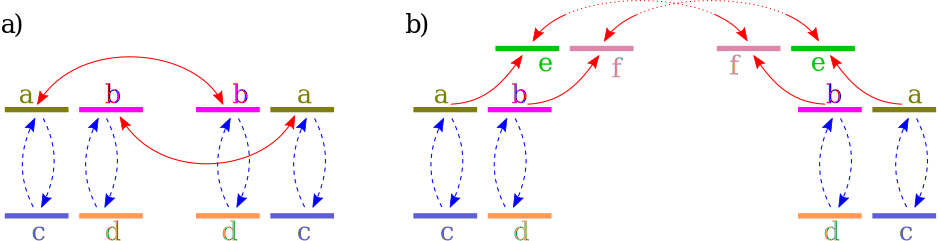
\includegraphics[width=0.9\linewidth]{figures/dipole_coupling_abab}
\caption[Couplage dipolaire entre niveaux de Rydberg différents]{Schéma du couplage dipolaire entre deux atomes dans des niveaux de Rydberg différents $a$ et $b$ : le couplage $ab-ab$ s'effectue au second ordre \textit{via} les niveaux $c$ et $d$. Le couplage $ab-ba$ peut s'effectuer à l'ordre 1(\textbf{a}), à l'ordre 2 via des niveaux intermédiaires $e$ et $f$(\textbf{b}), ou plus encore.}
\label{fig:Dip_abab}
\end{figure}


Lorsque les termes d'échange $A_{ab}$ deviennent comparables aux termes d'interaction directe $C_{ab}$, il peut être judicieux de diagonaliser le hamiltonien effectif \eqref{eq:MatrixCab_Aab}.
En effet, les états propres de celui-ci, qui sont les combinaisons symétrique et anti-symérique $(\ket{ab}\pm \ket{ba})/\sqrt{2}$, ne sont plus dégénérés et présentent respectivement des déplacements d'énergie
\begin{equation}
\label{eq:shift_abab}
\Delta E_{dd} = C_{ab} \mp A_{ab}.
\end{equation}

Afin d'illustrer les calculs d'interaction que nous venons de présenter, nous allons les appliquer à nos deux exemples que sont le niveau 60S et le niveau 50C.
Dans les deux cas, le calcul numérique consiste à diagonaliser le hamiltonien \eqref{eq:hamilt2atoms} à tous les ordres perturbatifs, en limitant l'espace de Hilbert à quelques centaines d'états de paire et sous l'approximation dipolaire.

\subsection{Les interactions dipolaires du niveau 60S}

\subsubsection*{L'interaction 60S-60S}
Dans le cas de l'état $\ket{60\text{S},60\text{S}}$, le terme dominant dans la somme \eqref{eq:VdW_aacd} permettant de calculer le coefficient de Van der Waals $C_{6,\text{60S60S}}$ est le coulage avec les paires $\ket{60\text{P}_j,59\text{P}_j}$.
Puisque $E_{60S}-E_{59P}>E_{60P}-E_{60S}$, le dénominateur du terme de couplage principal dans \eqref{eq:VdW_aacd} est positif.
On en déduit que l'interaction 60S-60S, et plus généralement toute interaction dipolaire nS-nS, est toujours répulsive.
%
\begin{figure}[!h]
\centering
\includegraphics[width=0.8\linewidth]{figures/VdW_60S60S}
\caption[Interaction dipolaire 60S-60S]{Déplacement en énergie de la paire 60S-60S par interaction de Van der Waals. Les différents sous-niveaux $\ket{60\text{P}_j,59\text{P}_j}$ sont représentés. L'échelle de couleur représente le carré de la projection sur l'état non perturbé $\ket{60\text{S},60\text{S}}$.
L'insert représente le déplacement d'énergie en échelle log-log et son ajustement sous la forme de Van der Waals.}
\label{fig:VdW_60s60s}
\end{figure}
%
Le calcul numérique de l'interaction 60S-60S et son ajustement sous la forme de Van der Waals, représentés en figure \eqref{fig:VdW_60s60s}, donnent la valeur
\begin{equation}
\label{eq:C660S}
C_{6,60S60S} = \numv{137.6(1)}\si{\giga\hertz\raiseto{6}\micro\meter}.
\end{equation}

L'ajustement de Van der Waals fonctionne très bien aux distances supérieures à $\sim\SIvv{3}{ \micro\meter}$.
Cependant, aux très courtes distances, la paire $\ket{60\text{S},60\text{S}}$ est très fortement couplée aux niveaux $\ket{60\text{P}_j,59\text{P}_j}$.
La distance critique est celle à laquelle le couplage dipolaire est aussi fort que la différence d'énergie entre les deux états de paire non perturbés, soit ici $\sim \SIv{2}{\giga\hertz}$.
En deçà de cette distance, les états propres du hamiltonien s'éloignent de plus en plus de l'état non perturbé $\ket{60\text{S},60\text{S}}$ et l'interaction évolue vers une interaction dipolaire résonante en $1/r^3$.

\subsubsection*{Les interactions 60S-$nl$}
Le niveau 60S interagit également avec des états de $n$ et $l$ différents.
Il convient alors, comme nous l'avons montré en \eqref{subsec:interaction_diff_levels}, de calculer non seulement les coefficients de Van der Waals $C_{ab}$, mais aussi les éléments de matrice d'échange $A_{ab}$.
De plus, il est possible ici d'avoir des termes d'échange dûs à un couplage dipolaire direct et qui varient donc en $r^3$.

\begin{figure}[h]
\centering
\includegraphics[width=0.8\linewidth]{figures/VdW_60S60P}
\caption[Interaction dipolaire 60S-60P$_{3/2}$]{Énergie de la paire 60S-60P$_{3/2}$ en présence de l'interaction dipolaire.
Les branches inférieure et supérieure correspondent respectivement aux superpositions symétrique et antisymétrique des deux niveaux de départ.
L'échelle de couleur représente le carré de la projection sur l'état non perturbé $\ket{60\text{S},60\text{P}_{3/2}}$.
La ligne pointillée représente le déplacement en énergie dû à l'interaction directe.
L'insert représente le déplacement d'énergie ainsi que le terme d'échange en échelle log-log et leurs ajustements en $1/r^6$ et $1/r^3$ respectivement.
}
\label{fig:VdW_60S60P}
\end{figure}

La figure \eqref{fig:VdW_60S60P} montre par exemple le résultat du calcul de l'interaction dipolaire pour une paire 60S-60P$_{3/2}$.
Aux grandes distances, l'état de la paire est projeté uniformément sur les deux superpositions symétrique et anti-symétrique.
Aux plus courtes distances cependant, d'autres niveaux contaminent la paire, qui n'est plus dans une superposition de $\ket{60\text{S}}$ et $\ket{60\text{P}_{3/2}}$.

En procédant dela même façon, on peut obtenir les coefficients d'interaction dipolaire pour n'importe quelle paire 60S-$nl$. La table \eqref{tab:VdWcoef_60S_nl} synthétise les résultats des calculs numériques pour plusieurs paires contenant le niveau 60S.

\begin{table}[h!]
	\centering
	\caption[Coefficients de Van der Waals 60S-nl]{Coefficients de Van der Waals pour les interactions de paire entre le niveau 60S et différents niveaux voisins $nl$.}
	\label{tab:VdWcoef_60S_nl}
	\begin{tabular}{c c c c}
		\toprule\midrule
%		\multicolumn{1}{c}{  }
%		&\multicolumn{1}{c}{\text{temps de vie à }\numv{0}\si{\kelvin}}
%		&\multicolumn{1}{c}{\text{temps de vie à }\numv{4.2}\si{\kelvin}}
%		&\multicolumn{1}{c}{\text{temps de vie à }\numv{300}\si{\kelvin}}
%		\\ 
		{ }&$C_6$ (\si{\giga\hertz\raiseto{6}\micro\meter}) & $A_6$ (\si{\giga\hertz\raiseto{6}\micro\meter}) & $A_3$ (\si{\giga\hertz\raiseto{3}\micro\meter})
		\\
		\midrule
		$60\text{S}_{1/2}, 60\text{S}_{1/2}$
		&$\SIv{137.6}{}$
		&$\SIv{0}{}$
		&$\SIv{0}{}$\\
		$60\text{S}_{1/2}, 57\text{S}_{1/2}$
		&$\SIv{-43.265}{}$
		&$\SIv{0.325}{}$
		&$\SIv{0}{}$\\
		$60\text{S}_{1/2}, 61\text{S}_{1/2}$
		&$\SIv{290.125}{}$
		&$\SIv{246.475}{}$
		&$\SIv{0}{}$\\
		$60\text{S}_{1/2}, 60\text{P}_{3/2}$
		&$\SIv{7.976}{}$
		&$\SIv{0}{}$
		&$\SIv{4.411}{}$\\
		\midrule
		\bottomrule
 	\end{tabular}
\end{table}



\subsection{Les interactions dipolaires du niveau 50C}
	
\noindent L'interaction dipolaire entre atomes de Rydberg de très grand moment cinétique est rendue plus complexe du fait de leur forte anisotropie.
En effet, l'interaction entre deux dipôles dépend de l'orientation relative de ceux-ci.
Dans le cas des niveaux $l=0$ tel que le 60S, le problème ne se posait pas car ces niveaux sont à symétrie sphérique.
Dès lors que l'on s'intéresse à l'interaction entre des niveaux à symétrie cylindrique, il est indispensable de savoir comment les atomes s'orientent l'un par rapport à l'autre.
L'interaction dipolaire entre atomes circulaires est encore compliquée par l'introduction d'un champ électrique extérieur, qui déplace et déforme les niveaux par effet Stark.
Le détail de l'interaction dipolaire entre atomes circulaires en présence d'un champ sera discuté au chapitre \ref{chapter:circsim}, mais nous prendrons le temps ici de développer la situation la plus simple :
celle de deux atomes dans le niveau 50C dont les deux orbites sont contenues dans le même plan, comme l'illustre la figure \eqref{fig:double_torus}.
%
\begin{figure}[!h]
\centering
\vspace{1em}
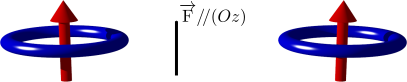
\includegraphics[width=.8\linewidth]{figures/double_torus.png}
\caption[Deux atomes circulaires côte à côte]{Représentation de deux atomes de Rydberg circulaires dont les orbites sont dans le même plan.
Les tores bleus représentent les orbites électroniques et les flèches rouges la direction du moment cinétique.
Si l'on imagine que le dessin est à l'échelle, alors les atomes sont ici séparés d'une distance d'environ \SIv{660}{\nm}.}
\label{fig:double_torus}
\end{figure}
%
Comme il a été dit en \ref{sec:circ_parabol}, les atomes de Rydberg circulaires ont besoin d'un champ électrique extérieur pour se stabiliser.
Nous imposerons donc un champ de \SIvvSym{1}{\V\per\cm}, qui définit l'axe de quantification, parallèle aux flèches rouges sur la figure \eqref{fig:double_torus}.

Les règles de sélection étant toujours valides, le couplage se fait \textit{a priori} à l'ordre deux, et l'équation \eqref{eq:VdW_aacd} permet d'en extraire le coefficient de Van der Waals comme nous l'avons fait pour l'interaction 60S-60S.
Cependant, l'équation \eqref{eq:Vdd_rr1r2} ne prend plus la même forme dans la base parabolique et le moment magnétique total $M$ de la paire atomique n'est plus conservé, ce que doit prendre en compte le calcul numérique.

\begin{figure}[!h]
\centering
\includegraphics[width=1\linewidth]{figures/VdW_50C50C_1Vcm}
\caption[Interaction dipolaire 50C-50C]{Déplacement en énergie de la paire 50C-50C placés côte à côte (cf fig\eqref{fig:double_torus}) par interaction dipolaire, sous un champ électrique de $\SIvv{1}{\V / \cm}$. L'échelle de couleur représente le carré de la projection sur l'état non perturbé $\ket{50\text{C} 50\text{C}}$ de l'état propre du hamiltonien qui le suit adiabatiquement.
Le comportement dévie franchement de la forme de Van der Waals en $1/r^6$ dès que la distance interatomique est inférieure à $\SIv{10}{\micro\meter}$.
%Aux très courtes distances, le couplage vers d'autres niveaux atomiques devient très fort et l'énergie d'interaction}
}
\label{fig:VdW_50C50C_1Vcm}
\end{figure}

La figure \eqref{fig:VdW_50C50C_1Vcm} présente le résultat du calcul numérique.
Aux grandes distances, l'énergie d'interaction varie bien en $1/r^6$ comme on l'attend, avec un coefficient de Van der Waals 
\begin{equation}
\label{eq:C6_50C50C}
C_{6,50C50C}(\SIvv{1}{V/cm}) = \SIv{483.17}{\GHz\raiseto{6}\um}.
\end{equation}
Mais dès que les atomes se rapprochent à une distance inférieure à $\SIvv{10}{\um}$, l'énergie d'interaction varie en $1/r^3$ jusqu'à très courte distance.
En effet, lorsque l'interaction dipolaire devient suffisamment forte, le champ électrique extérieur ne suffit plus à définir le plan des orbites, et le niveau de paire est perturbé.
C'est ce que l'on retrouve sur la coloration de la courbe : à une distance critique de l'ordre de $\SIvv{10}{\um}$ le niveau de la paire s'éloigne du niveau non perturbé $\ket{\mathrm{50C50C}}$.
La paire est alors dans un état superposé de plusieurs $\ket{nmk,n'm'k'}$, entre lesquels apparaissent des couplages dipolaires résonants en $1/r^3$.
Ce problème sera traité en détail dans le chapitre \ref{chapter:circsim}, lorsque nous nous intéresserons aux conditions dans lesquelles les interactions entre atomes circulaires sont les plus avantageuses pour la simulation quantique.

Si l'on approche encore les deux atomes, à des distances inférieures à \SIvv{2}{\um}, la base des états propres du hamiltonien de paire devient très différente de la base des états non perturbés.
Il est alors très difficile de décrire simplement l'interaction dipolaire.

\section*{Conclusion}
\noindent Nous avons dans ce chapitre présenté les caractéristiques physiques principales des atomes de Rydberg alcalins.
Nous avons utilisé la théorie du défaut quantique afin de décrire les niveaux de Rydberg de faible moment cinétique.
Ceux-ci dévient en effet du modèle de l'atome d'hydrogène par les effets de pénétration et de polarisabilité du c\oe ur atomique, ce que permet de corriger le défaut quantique.
Ainsi nous avons pu calculer décrire le niveau 60S, en donnant la forme de sa fonction d'onde, sa taille et sa durée de vie radiative à différentes températures.

Nous nous sommes ensuite intéressés aux niveaux de Rydberg circulaires, qui semblent être de meilleurs candidats pour la simulation quantique grâce à leur temps de vie plus long.
La théorie du défaut quantique n'est plus nécessaire pour décrire les niveaux circulaires.
Cependant, l'introduction de la base des états paraboliques est d'une grande aide à leur description, en particulier en présence d'un champ électrique.
Nous avons ainsi pu décrire le niveau de Rydberg circulaire 50C, qui présente un temps de vie à température nulle de presque \SIvv{30}{\ms}.

En dernier lieu, nous avons vu comment les atomes de Rydberg interagissent entre eux par interaction dipolaire.
\`A grande distance, l'interaction dipolaire entre deux atomes de Rydberg prend la forme de Van der Waals avec une dépendance en $C_6/r^6$, où $r$ est la distance entre les deux atomes.
Nous avons pu déterminer les coefficients de Van der Waals $C_6$ pour l'interaction entre une paire d'atomes dans les niveaux $\ket{\text{60S60S}}$, $\ket{\text{60S,nl}}$ et $\ket{\text{50C50C}}$, en diagonalisant à chaque fois le hamiltonien complet du système pour toutes les distances $r$.
Aux distances très courtes, lorsque l'interaction dipolaire devient comparable aux différences d'énergie entre les niveaux de Rydberg, les niveaux de Rydberg se mélangent et l'interaction dipolaire ne peut plus être traitée simplement.

Les expériences que nous avons menées portent sur l'étude de l'interaction dipolaire entre atomes de Rydberg.
Il nous a fallu pour cela mettre en \oe uvre un dispositif expérimental que nous présentons dans le prochain chapitre.% \eqref{chapter:setup_coldatoms_Rydberg} .

%Plus particulièrement, nous avons étudié l'interaction dipolaire au sein d'un nuage dense d'atomes dans le niveau 60S, et nous avons 

%Les particularités de l'interaction dipolaire entre niveaux de très grand $l$ sera traitée au chapite \ref{chapter:circsim}.